\documentclass[a4paper,fleqn]{cas-sc}

\usepackage[numbers,sort&compress]{natbib}
\usepackage{graphicx}
\usepackage{amsmath,amssymb,amsfonts}
\usepackage{booktabs}
\usepackage{microtype}
\usepackage{placeins}
\usepackage{float}
\usepackage{url}
\usepackage{xcolor}
\makeatletter
\DeclareRobustCommand{\rev}[1]{{\color{red}\def\@citecolor{black}\def\@linkcolor{red}\def\@urlcolor{red}#1}}
\let\unmarkedcite\cite
\renewcommand{\cite}[1]{{\color{black}\def\@citecolor{black}\unmarkedcite{#1}}}
\makeatother
\pdfstringdefDisableCommands{\def\rev#1{#1}}
\graphicspath{{figure/}}
\urlstyle{same}
\raggedbottom
\renewcommand{\topfraction}{0.95}
\renewcommand{\bottomfraction}{0.95}
\renewcommand{\textfraction}{0.05}
\renewcommand{\floatpagefraction}{0.80}

% Support standard figure placement options such as [t], [tbp], and [H] in CAS.
\ExplSyntaxOn
\keys_define:nn { cas / fig }
  {
    t .code:n = { \tl_set:Nn \l_fig_pos_tl { t } },
    tbp .code:n = { \tl_set:Nn \l_fig_pos_tl { tbp } },
    H .code:n = { \tl_set:Nn \l_fig_pos_tl { H } }
  }
\ExplSyntaxOff

\makeatletter
\AtEndDocument{\clearpage\immediate\write\@auxout{\string\csxdef{lastpage}{\number\numexpr\value{page}-1\relax}}}
\makeatother

\begin{document}
\let\WriteBookmarks\relax
\def\floatpagepagefraction{1}
\def\textpagefraction{.001}

% Leave the running title empty so that figure and text pages have no title header.
\shorttitle{}
\shortauthors{G. Yang et~al.}

\title[mode=title]{\rev{Cross-context ordering and prioritization of UPR-associated transcriptional responses}}

\author[1]{Guang Yang}
\credit{Conceptualization, Methodology, Formal analysis, Visualization, Writing -- original draft}

\author[1]{Qi Yu}
\credit{Data curation, Software, Formal analysis, Validation, Visualization}

\author[1]{Renyu Yang}
\credit{Methodology, Software, Formal analysis, Validation, Writing -- review and editing}

\author[1]{Chunxue Shao}
\credit{Data curation, Investigation, Validation, Visualization, Writing -- review and editing}

\author[1]{Zongnan Lyu}
\credit{Data curation, Formal analysis, Validation, Visualization, Writing -- review and editing}

\author[1]{Ziheng Wang}[orcid=0000-0002-3953-0493]
\cormark[1]
\ead{wangzh654@nenu.edu.cn}
\credit{Conceptualization, Supervision, Project administration, Methodology, Writing -- review and editing}

\affiliation[1]{organization={Division of Computational Biology, Chinese Center of Exercise Epidemiology, Northeast Normal University},
                  city={Changchun},
                  postcode={130024},
                  state={Jilin},
                  country={China}}

\cortext[1]{Corresponding author}

\begin{abstract}
\noindent \rev{Single-cell perturbation screens reveal context-dependent responses, but it is unclear which response information transfers across experiments.} \rev{We harmonized twelve transcriptional scores across genetic and chemical screens to ask whether response ordering can guide candidate perturbation selection across experimental contexts.} \rev{Matched-state models and an aggregate gene-priority score did not improve independent-study prediction.} \rev{An exploratory comparison of all twelve axes identified conserved unfolded protein response (UPR) effect ordering in Adamson K562 and unstimulated Frangieh melanoma data (Spearman $\rho=0.823$ and 0.674; both false-discovery-rate-adjusted $q<0.01$).} \rev{Exact target-expression composition controls retained these associations.} \rev{A subsequent source-frozen test in 438 Replogle RPE1 perturbations confirmed signed UPR ordering ($\rho=0.378$, $95\%$ interval $[0.289,0.461]$).} \rev{Fixed top-twenty and top-ten priorities exceeded matched-background UPR effects by 0.329 and 0.573 control standard deviations, respectively (all three Holm-adjusted $P\leq0.0004$).} \rev{An independent HepG2 screen retained ordering in 417 supported perturbations ($\rho=0.403$, $95\%$ interval $[0.313,0.489]$; Holm-adjusted $P=0.00050$).} \rev{Its complete top-ten/top-twenty lists lacked primary cell support, but a separately specified lower-support sensitivity gave positive-effect precision of 0.80/0.75 and exceeded matched random-module priorities.} \rev{Simple UPR-effect sorting remained competitive.} \rev{These results support reproducible ordering of transcriptional program responses across experimental contexts and candidate perturbation prioritization for a specified RNA readout.} \rev{Complete-list primary utility remains coverage-limited.}

\end{abstract}

\begin{keywords}
single-cell perturbation \sep \rev{unfolded protein response} \sep \rev{cross-study validation} \sep Perturb-seq \sep \rev{gene prioritization}
\end{keywords}

\maketitle
\hypersetup{pdfauthor={Guang Yang, Qi Yu, Renyu Yang, Chunxue Shao, Zongnan Lyu, Ziheng Wang}}

\section{Introduction}

Cell identity is maintained by coupled transcriptional, regulatory, signalling, metabolic and chromatin processes. Perturbing one component can move a cell towards a different phenotype, but the same intervention may be ineffective or redirect the response when applied from another baseline state. This state dependence is central to differentiation, reprogramming and treatment response, as illustrated by transcription-factor reprogramming, direct lineage conversion and network-guided cell engineering.~\cite{takahashi2006,cahan2014,rackham2016,kamimoto2023} \rev{Single-cell perturbation experiments make it possible to ask a more specific question: which components of a transcriptional response remain predictable when the experiment or cellular context changes?}

\rev{Early Perturb-seq and CRISP-seq studies established guide-resolved transcriptional screening, and subsequent approaches expanded its scale and perturbation capture.~\cite{dix2016,adamson2016,jaitin2016,datlinger2017,gasperini2019,schraivogel2020}} \rev{Genome-scale CRISPR interference, combinatorial CRISPR activation and multiplexed drug profiling now measure complementary forms of response variation.~\cite{replogle2022,norman2019,mcfarland2020}} \rev{Models including scGen, compositional perturbation autoencoders, chemCPA and GEARS address prediction across unmeasured conditions or perturbations.~\cite{scgen2019,cpa2023,chemcpa2022,gears2024}} \rev{Their evaluation must distinguish the transfer of an intervention-specific response from predictable variation shared by many perturbed cells.} \rev{Systema demonstrated that systematic expression variation can dominate common prediction metrics and obscure this distinction.~\cite{systema2026}} \rev{An accurate average expression profile therefore need not identify which perturbation will produce the strongest response on a specified biological program.}

\rev{Two forms of information could support such transfer.} \rev{Matched control profiles describe the cellular context in which a response is measured, whereas a perturbation measured in one experiment provides direct information about its response in another.} \rev{These inputs address different questions: context-based prediction of an unmeasured response and transport of an already characterized intervention.} \rev{Lineage tracing offers an additional test because it links measured earlier states to later relatives, rather than assigning pretreatment states to unrelated endpoint cells.~\cite{weinreb2020,biddy2018,kester2018,schaff2024}} \rev{Keeping these settings separate is necessary to determine whether baseline-state features contribute predictive information and whether a conserved molecular response supports practical gene prioritization.}

\rev{Here we harmonized twelve transcriptional scores across Replogle, Norman and MIX-Seq and evaluated their transport with entire studies held out.} \rev{Discovery-only aggregate priorities did not validate in separately generated Adamson and Frangieh screens, whereas an exploratory comparison of all twelve axes identified UPR-associated perturbation-effect ordering across these studies.} \rev{This observation motivated source-frozen evaluation in held-out RPE1 expression data and a subsequent unused HepG2 experiment, with candidate identities, RNA readout and evaluation metrics fixed before expression scoring.} \rev{Comparisons with simple source effects, generic perturbation strength and matched random-module priorities distinguish reproducible program ordering from useful candidate selection.} \rev{Together, these analyses evaluate reproducible ordering of transcriptional program responses across experimental contexts and its use in candidate perturbation prioritization for a specified molecular readout.} \rev{The independent-screen tests assess the transport of measured responses; their cell-support requirements determine whether complete candidate lists can be evaluated.}

\section{Materials and Methods}

\subsection{\rev{Sources and a common measured gene space}}

\rev{Only public data were used.} \rev{The primary harmonization combined Replogle K562 CRISPR interference (CRISPRi; Figshare article 20029387), Norman K562 CRISPR activation (CRISPRa; GSE133344) and chemical MIX-Seq profiles (Figshare version 3).~\cite{replogle2022,norman2019,mcfarland2020}} \rev{Independent-study validation used Adamson K562 CRISPRi (GSE90546, GSM2406681) and Frangieh melanoma CRISPR knockout (SCP1064), with unstimulated, interferon-$\gamma$ and co-culture conditions distinguished.~\cite{adamson2016,frangieh2021}} \rev{Replogle RPE1 provided a held-out cellular context from the same study as the K562 discovery data; it was not counted as an independent study.} \rev{The published Schaff melanoma lineage experiment (GSE253739) provided measured states before a second treatment and subsequent lineage-linked profiles.~\cite{schaff2024}} \rev{Original count matrices were read without modification; accessions, file checksums, retained cell identifiers and measurement schemas accompany the analysis.}

\rev{The intersection of measured gene symbols in the five primary transcriptomic sources contained 7,848 genes and was fixed from feature metadata before external effect evaluation.} \rev{Counts for duplicated symbols were summed before transformation.} \rev{Each cell was normalized by the count sum over this common universe, followed by $\log(1+10^4x/L)$.} \rev{Unmeasured genes were not imputed as zero.} \rev{Scores comprised the existing signed apoptosis-, proliferation- and stress-associated short modules and nine Hallmark expression summaries: UPR, E2F, G2/M, p53, TNF/NF-$\kappa$B, interferon-$\gamma$, mTORC1, oxidative phosphorylation and hypoxia.~\cite{liberzon2015}} \rev{Positive-member means were calculated after normalization; negative-member means were subtracted for the signed short modules.} \rev{The retained gene sets and their coverage are provided in Supplementary Data.} \rev{These are overlapping RNA-expression summaries, not independent pathways, functional event probabilities or fitted biochemical activities.}

\rev{Source QC retained 276,108 Replogle cells and 104,507 Norman cells.} \rev{Preferred matched controls were selected in MIX-Seq before chemical-task construction; its chemical branch contained 120,003 cells.} \rev{Technical GEM groups were retained as within-experiment partitions.} \rev{Norman and Replogle K562 are separate studies in the same cell line, and GEM groups do not constitute independent biological contexts.} \rev{Assay-specific catalogues used different response-selection rules and are documented separately in Supplementary Notes S1--S6; their cell and task totals are not denominators of the harmonized analyses.}

\subsection{\rev{Study-held-out response and sampling-precision prediction}}

\rev{Eligibility required at least ten treated cells in a perturbation--context unit and sixty matched controls, without filtering on effect magnitude, significance or response agreement.} \rev{Each control pool was partitioned into disjoint subsets A, B and C.} \rev{Control C supplied context means and variances; independently partitioned treated A and B cells and their matching control subsets supplied response estimates A and B.} \rev{Thus the context features and target contrasts did not share control cells.} \rev{Ten deterministic partitions were evaluated, with the first designated primary and the others used as sensitivity analyses.}

\rev{For each held-out study, predictor scaling, ridge fitting and penalty selection used only the other two studies.} \rev{Inner leave-study-out evaluation selected the penalty jointly across all twelve raw-score outputs from $\{0.01,0.1,1,10,100\}$; core-module errors were evaluated without retuning.} \rev{Training studies received equal weight.} \rev{Predictors comprised context state, cell/library support, a measured pilot response A and their specified combinations; outcomes were response B or log squared A--B disagreement.} \rev{Zero response, training-study mean, unshrunk pilot A and an analytic sampling-variance estimate provided simple baselines.} \rev{The pilot setting explicitly assumes an observed response in a disjoint cell sample; it is distinct from predicting an entirely unmeasured perturbation.}

\rev{Responses remained in raw common-score units for prediction; program-wise and joint errors were both retained.} \rev{Incremental-state contrasts used intervention-, context- and crossed-cluster bootstrap resampling conditional on fixed predictions and cell partitions.} \rev{MIX-Seq context resampling retained complete cell lines; Norman additionally used deterministic anchor-gene clusters to assess dependence among combinations sharing genes.} \rev{These intervals do not represent between-study biological replication or complete model-refitting uncertainty.} \rev{A target-mutation check verified that changing held-out response B altered neither predictions nor tuning.} \rev{Matched controls were contemporaneous endpoint controls, rather than paired pretreatment measurements of the treated cells.} \rev{A--B disagreement measures random-cell sampling precision, not independent-experiment reproducibility.}

\subsection{\rev{Discovery-only gene priorities and independent-study validation}}

\rev{The initial candidate score was defined in Replogle without external response values.} \rev{For each gene, the dominant absolute shift among the three short modules defined its program and sign.} \rev{Priority was the absolute standardized shift multiplied by nonnegative across-GEM response cosine and divided by one plus the norm on the other two modules.} \rev{Eligibility required at least 100 discovery cells and three GEM groups, without a response-significance gate.} \rev{Fixed external support criteria produced 30 Adamson genes and 19 Frangieh genes in the unstimulated condition; 17 were measurable in co-culture.} \rev{The top ten were compared with the remaining eligible genes using sign-aligned external program effects.} \rev{Absolute dominant-program magnitude, total response magnitude, technical agreement, control expression, cell count and generic essentiality were evaluated on identical available panels.} \rev{Essentiality was the negative mean available Chronos effect across DepMap Public 24Q4 cell lines.~\cite{depmap2024,dempster2021}} \rev{Unavailable comparator values were retained as missing and coverage was reported.}

\rev{After the initial priority test, all twelve source-versus-external signed-axis associations were evaluated in Adamson and the three Frangieh conditions.} \rev{Two-sided gene-label permutation tests were adjusted jointly across all 48 comparisons by Benjamini--Hochberg correction.} \rev{Gene bootstraps estimated conditional rank-correlation intervals.} \rev{The UPR follow-up was selected from this exploratory family, rather than retrospectively designated as the original primary endpoint.} \rev{Direct copying of the twelve-dimensional source effect was also compared with zero and the mean discovery response.} \rev{Gene-level, equal-cell, single-guide and minimal covariate sensitivities tested the dependence of the associations on individual genes, sampling support and generic response features.}

\rev{For UPR composition controls, the targeted gene was removed from the score numerator when it belonged to the UPR set, and matched-control means and standard deviations were recalculated.} \rev{A separate exact correction excluded the target's raw counts from the common-library denominator for every targeted gene measured in that universe, including targets outside the UPR gene set.} \rev{Every log-expression term was recomputed; no aggregate-score rescaling substituted for this correction.} \rev{The complete 48-test family was retained when the four UPR tests were replaced by their corrected sensitivity statistics.} \rev{Paired comparisons between melanoma contexts used the same shared genes and multiplicity correction across the twelve axes and two context contrasts.}

\subsection{\rev{Source-frozen UPR prioritization in RPE1}}

\rev{The targeted RPE1 evaluation was specified after the exploratory external UPR finding and before reading RPE1 expression outcomes.} \rev{Measurement metadata defined a 6,780-gene common universe and 90 shared UPR members for both K562 and RPE1.} \rev{All five-source analyses retained their original 7,848-gene universe and 91 UPR members.} \rev{K562 eligibility required at least 100 retained cells and three GEM groups each containing at least five target cells; RPE1 eligibility required at least 100 published cells and three GEM labels.} \rev{This metadata-only intersection contained 438 genes.} \rev{A stricter RPE1 support rule, with at least five cells in each of three GEM groups, retained 390 genes as a sensitivity population.} \rev{The locked primary extraction yielded 97,065 cells (85,580 treated and 11,485 controls), with no unscorable common libraries.} \rev{RPE1 lacked an available doublet/QC flag; the published roster was retained with finite positive recorded UMI counts; unscorable common-library zeros were recorded after extraction without changing the locked gene panel.}

\rev{For gene $g$, the UPR effect was the target-cell-count-weighted mean of matched-GEM treated-minus-control contrasts, standardized by the applicable global control standard deviation.} \rev{All 105 follow-up readouts (UPR, one hundred random modules, three short modules and E2F) excluded their own targeted member where applicable and recalculated matched-control standardization; the original five-source scores were unchanged.} \rev{Let $d_g$ be this source standardized effect and $f_g$ the fraction of supported source GEM groups with a positive contrast.} \rev{The source-only priority was
\begin{equation}
{S_g=\max(d_g,0)f_g.}
\end{equation}
One descending ranking, with $d_g$ and then gene symbol breaking ties, defined nested top-ten and top-twenty lists.} \rev{No prediction weights were fitted to RPE1.} \rev{Comparator rankings used positive UPR effect alone, generic three-module response magnitude, DepMap essentiality, source control target expression and source cell count; annotation-derived genome-wide response significance was an additional comparator, rather than an unmodified author-provided significance value.}

\rev{Each top-twenty gene was matched before outcome access to five distinct background genes, without replacement across the resulting background list.} \rev{Matching used standardized log source cell count, control target expression, generic three-module magnitude and essentiality, with equal-weight Euclidean distance and deterministic ties.} \rev{Top-ten tests used the corresponding subsets.} \rev{Covariate availability and balance were recorded before validation; incomplete lists were not silently shortened.} \rev{The primary test family comprised signed source--RPE1 UPR Spearman correlation and top-twenty and top-ten mean RPE1 UPR effects relative to their frozen backgrounds.} \rev{Two-sided permutation tests used expression-by-count strata for correlation and exchangeable roles within six-gene matched sets for enrichment; the three $P$ values were Holm-adjusted.} \rev{The tests used 10,000 permutation draws, and 2,000 whole-gene or intact-matched-set bootstrap draws supplied conditional intervals.}

\rev{One hundred random 90-gene modules were fixed using source-control expression and detection bins, excluding UPR genes.} \rev{Module membership, source effects, rankings, comparator inputs and matches were hashed before RPE1 extraction.} \rev{The same own-member numerator exclusion was applied to every random module in treated and control cells.} \rev{The random modules tested response-correlation specificity and the ability of their source-frozen priorities to select high RPE1 UPR effects.} \rev{Missing-covariate lists and the effective number of evaluable modules were reported.} \rev{A separately fixed complete-covariate sensitivity used the same measurable candidate population for UPR, random modules and comparators.} \rev{Additional checks included exact all-target denominator exclusion, 200 without-replacement resamples of one hundred target cells per gene in each context with the original matched-GEM control means and target-specific control standard deviations retained, stricter GEM support and shared-GEM wild-bootstrap uncertainty.} \rev{Technical wild draws used a shared Rademacher sign per GEM on gene-specific centered weighted GEM residuals, retained missing GEMs as unobserved and used identical weights across methods; control standard deviations remained fixed.} \rev{The follow-up tests an ordinal molecular-response priority in a held-out cell context, not prospective experimental efficacy or a biological control node.}

\rev{We further divided all 438 shared genes into five groups ordered by their signed K562 UPR effect, breaking ties by gene symbol, with 88, 88, 88, 87 and 87 genes.} \rev{Group membership was fixed from K562; RPE1 effects did not define the boundaries.} \rev{We estimated group means, medians, positive-effect fractions, the Q5--Q1 mean contrast, Kendall's rank trend and the mean-effect change per quintile.} \rev{Whole-gene and shared-GEM resampling retained the fixed source groups.} \rev{Simultaneous max-$t$ intervals assessed the four adjacent mean contrasts; frequencies of fully ordered means were descriptive sensitivity measures.} \rev{A positive overall trend was not interpreted as a strictly monotonic increase.}

\rev{For the existing source-frozen lists, Precision@$K$ was the fraction of RPE1 effects above zero, and normalized discounted cumulative gain (NDCG@$K$) used linear relevance $\max(d_g^{\mathrm{RPE1}},0)$ with a $\log_2(r+1)$ rank discount.} \rev{Zero was a fixed matched-control reference, not a fitted validation threshold.} \rev{We evaluated $K=10,20$ against the unchanged positive-source-UPR ranking, control expression, essentiality, generic response magnitude, cell support, uniform random rankings and the original one hundred expression/detection-matched random-module rankings.} \rev{Fair method comparisons used the same 370-gene complete-comparator population; all-438 results and unavailable literal lists were retained separately.} \rev{Shared gene weights preserved overlap between rankings.} \rev{Gene-bootstrap NDCG-difference intervals conditioned on the observed common ideal gain; technical-GEM draws recalculated effects, signs and ideal gain.} \rev{Three quintile tests and four priority-minus-unweighted-UPR Precision/NDCG comparisons formed one seven-test Holm family.} \rev{Additional reference distributions and sensitivity intervals were descriptive.} \rev{These outcomes had already been analysed for Hallmark UPR, so the added tests were retrospective robustness evaluations, rather than a new independent validation.}

\rev{A separate sequencing-depth diagnostic fitted the fixed-library ninety-gene Hallmark outcome to source and RPE1 target-cell mean log1p recorded UMI counts in all 438 genes.} \rev{The unchanged top-ten/top-twenty and matched-background lists were compared on the model residuals; two thousand shared whole-gene bootstrap draws refitted the depth model and recomputed weighted group means.} \rev{This was a descriptive conditional comparison, with no new ranking, threshold or adjusted Precision endpoint.}

\rev{Additional robustness analyses used functional definitions and evaluation metrics fixed before their corresponding calculations.} \rev{Gene Ontology (GO) readouts represented ER protein folding (GO:0034975), ER-associated degradation quality control (ERAD; GO:0036503), protein targeting to the ER (GO:0045047) and integrated stress response (ISR; GO:0140467).~\cite{go2000,go2026}} \rev{Alternative UPR definitions used Reactome R-HSA-381119.4 and GO:0030968.~\cite{reactome2024}} \rev{Human protein-product annotations were propagated through \texttt{is\_a}/\texttt{part\_of}, excluding \texttt{NOT} annotations, and mapped by unambiguous approved HGNC symbols.} \rev{Full, approved-symbol-Hallmark-disjoint and between-functional-module-unique memberships produced sixteen fixed expression summaries.} \rev{Their means quantify annotated RNA abundance, rather than protein-folding, ERAD, translocation or kinase activity.} \rev{Membership, overlap, coverage and annotation versions are reported in Supplementary Note S13.} \rev{Functional target membership was tabulated separately; small or absent target strata were not treated as replicated functional classes.}

\rev{All new readouts used the same 6,780-gene library and fixed 438/30/19/19/17-gene panels.} \rev{The original ninety-member Hallmark score remained the reference.} \rev{The full approved-symbol Hallmark membership was removed before intersecting disjoint readouts with measured genes; approved-symbol mapping identified 94 measured exclusions, including four aliases absent from the frozen ninety-member score.} \rev{An identifier-coverage sensitivity restored these four genes without changing the original score, cohorts or candidate lists.} \rev{Real readouts used exact own-target numerator and library-denominator exclusion in treated and control cells.} \rev{Matched-size/expression/detection random-readout calibration used a separate fixed-library analysis, applying identical own-member numerator exclusion to both real and random sets.} \rev{Eight readout families each had one hundred source-control-matched random sets, fixed before response evaluation.} \rev{Real exact-normalization results were never compared directly with fixed-library null results.}

\rev{Signed rank associations across sixteen readouts and five comparisons formed an eighty-test BH family.} \rev{Gene bootstraps used 4,999 draws and two-sided gene-label permutations used 19,999 draws; resampling retained repeated-context gene identity.} \rev{Direction tests preserved both sign marginals, and chance-adjusted agreement was reported alongside raw concordance.} \rev{Conditional technical-GEM and equal-cell analyses assessed measurement sensitivity.} \rev{Four fixed minimal-covariate checks per association were retained separately from the primary family.} \rev{The eighty association tests and seven quintile/ranking tests were also pooled in a global BH sensitivity.} \rev{Sequencing-depth diagnostics separately conditioned on source and validation target-cell mean log1p UMI counts or common-library counts.} \rev{The sixteen curated readouts and the fixed-library ninety-gene Hallmark reference were assessed across all five comparisons in one 170-test BH sensitivity family.} \rev{These captured-RNA depth measures can reflect perturbation-induced RNA content as well as sequencing support, so the adjustment was treated as a conditional diagnostic rather than pure technical deconfounding.} \rev{Module and ranking checks used study outcomes previously examined for Hallmark UPR and were treated as retrospective robustness analyses, rather than a new independent validation.} \rev{Alternative-definition source rankings were frozen before reading their newly scored RPE1 responses; the existing top-ten/top-twenty lists were not replaced.}

\rev{A further cross-study test used the separately generated HepG2 CRISPRi screen from GSE264667.~\cite{nadig2025}} \rev{The ninety UPR members, original source priorities, literal top-ten/top-twenty lists, comparator rankings and one hundred matched-module source priorities were fixed before HepG2 expression scoring.} \rev{The published matrix contained 145,473 cells; the retained source-target/control panel comprised 37,996 target cells and 4,976 non-targeting controls.} \rev{All ninety UPR genes were measured.} \rev{The validation library used the 6,523 assayed members of the frozen 6,780-gene universe; the 257 unavailable features were not zero-imputed.} \rev{Exact target-count denominator and own-member numerator exclusion were applied to treated and control cells, using matched controls within 56 technical GEM groups and target-specific global control standard deviations.} \rev{The fixed-library measurement was retained as a sensitivity.} \rev{This was a separate experiment reported by an overlapping research group, rather than independent-laboratory replication.}

\rev{The primary support rule required thirty target cells and sixty controls, retaining 417 of the 438 source genes.} \rev{Metadata showed seventeen GBF1 cells and twenty-four ALG14 cells, so neither complete literal list met primary support; missing members were not replaced.} \rev{Before expression outcomes were calculated, a separately documented ten-cell sensitivity was fixed to assess all 438 genes, while the original hundred-cell sensitivity retained 106.} \rev{These sensitivities did not replace the primary support criterion.} \rev{Five primary hypotheses comprised signed source--validation rank association, top-ten/top-twenty signed-effect gaps against eligible nonselected genes, and two weighted-minus-simple-UPR NDCG contrasts.} \rev{Unestimable statistics remained missing, with $P=1$ only as a correction placeholder in the five-test Holm family.} \rev{Tests used 10,000 gene permutations and intervals used 4,999 whole-gene bootstrap draws.} \rev{Shared-GEM perturbations supplied 2,000 conditional technical sensitivity draws, with source effects and control standard deviations fixed.}

\rev{Precision used the unchanged positive-effect threshold and NDCG used the same linear gain and rank discount.} \rev{The seven named rankings were compared on the same frozen 370-gene complete-source-covariate frame; validation support and literal-list availability were reported for every method.} \rev{All one hundred matched-module source rankings predicted the same HepG2 UPR outcome, alongside 10,000 uniform orderings.} \rev{Their finite upper-tail fractions were descriptive calibrations, not independent biological replications or additional confirmatory tests.} \rev{Full specifications, support accounting and results are provided in Supplementary Note S14.}

\subsection{\rev{Independent lineage analysis and supporting assay checks}}

\rev{The Schaff author count object supplied 74,325 melanoma cells; 39,011 had unambiguous assigned lineage labels.~\cite{schaff2024}} \rev{Earlier-state features were reconstructed from counts using the frozen twelve axes, without reusing the original PCA or outcome analyses.} \rev{Parent profiles preceded the second treatment; descendant program levels, rather than parent-subtracted changes sharing noisy inputs, were prediction outcomes.} \rev{Five outer and four inner folds retained whole ancestral lineages.} \rev{Training-only scaling and tuning compared state-augmented ridge with treatment/count models, treatment means and calibrated parent persistence.} \rev{Each lineage received total weight one.} \rev{The primary parent/descendant support rule (three/two cells) retained 257 tasks from 166 lineages; stricter ten/five-cell thresholds retained 85 tasks from 52 lineages.} \rev{The outcome axes were the three short modules, scaled by each outer-training axis standard deviation.} \rev{All 249 whole-lineage bootstrap draws repeated model fitting, tuning and comparator selection within the fixed grouped fold structure.} \rev{Descendant sampled-cell count is post-sampling information, so this is a conditional measured-response analysis.}

\rev{Assay-specific supporting analyses retained the original LARRY sampling simulation, nested MIX-Seq comparison and intervention-choice analysis, Norman additive-response contrasts and MultiPerturb non-targeting-control tests.} \rev{Their full definitions and results appear in Supplementary Notes S1--S7.} \rev{Unsupported MultiPerturb roles were excluded; endpoint-similarity graphs and duration contrasts remained exploratory supplementary descriptions.} \rev{Missing combination or functional assays were not treated as negative biological evidence.}

\subsection{\rev{Software and reproducibility}}

\rev{Analyses and figures used R; the count-level nested scVI benchmark used Python, scvi-tools 1.4.3 and PyTorch 2.5.1 on CPU.} \rev{Frozen gene memberships, eligibility masks, cell partitions, source rankings, validation effects, prediction outputs, random-module definitions and software records accompany the reproducibility archive.} \rev{Raw source matrices are referenced by accession and checksum rather than duplicated.} \rev{Numerical verification concerns the stated measurements and calculations; it does not substitute for independent biological replication.}

\section{Results}

\subsection{\rev{A common measurement space separates study transfer from within-experiment precision}}

\rev{We first constructed a common expression space for the response components that could be measured in every primary source and independent-study validation dataset.} \rev{Metadata-only intersection retained 7,848 unique genes and twelve fixed transcriptional scores.} \rev{The three discovery resources contributed 276,108 Replogle cells, 104,507 Norman cells and 120,003 chemical MIX-Seq cells.} \rev{Their biological coverage differed: the two genetic screens were separate K562 experiments, whereas MIX-Seq included many cancer cell lines.} \rev{We therefore treated study transfer, cellular-context transfer and randomized-cell repeatability as distinct outcomes.}

\rev{Response-independent support rules retained 2,151 Replogle gene--GEM units from 358 genes, 2,180 Norman condition--GEM units from 280 conditions and 527 MIX-Seq drug--context units from thirteen drugs and 109 cell lines.} \rev{These 4,858 units do not constitute 4,858 independent experiments.} \rev{Disjoint control subsets separated context-state features from response anchors, and disjoint treated subsets separated pilot and evaluation responses (Supplementary Note S8).} \rev{This construction made it possible to test the incremental value of control-state features without selecting the evaluated units for large or reproducible effects.}

\subsection{\rev{Matched control state does not improve the tested cross-study response models}}

\rev{Holding out an entire study did not establish a transferable gain from the measured control state.} \rev{Across the three short modules, adding control-state features to the pilot-response model increased RMSE from 0.2021 to 0.2298 in MIX-Seq, from 0.0887 to 0.0954 in Norman and from 0.1463 to 0.1470 in Replogle (Fig.~\ref{fig:transfer}).} \rev{Crossed intervention/context bootstrap intervals for the differences were $[0.0181,0.0398]$, $[0.00529,0.00798]$ and $[-0.000635,0.00206]$, respectively.} \rev{The twelve-axis analysis gave the same primary ordering; adding state worsened error in all ten cell partitions for MIX-Seq and Norman and nine of ten for Replogle.} \rev{In MIX-Seq, copying the unshrunk pilot response was substantially better than either transferred ridge model: twelve-axis RMSE was 0.0495, compared with 0.1086 for pilot-only ridge.} \rev{Thus a measured response in the same condition was more informative than the attempted shared state correction.}

\begin{figure}[tbp]
\centering
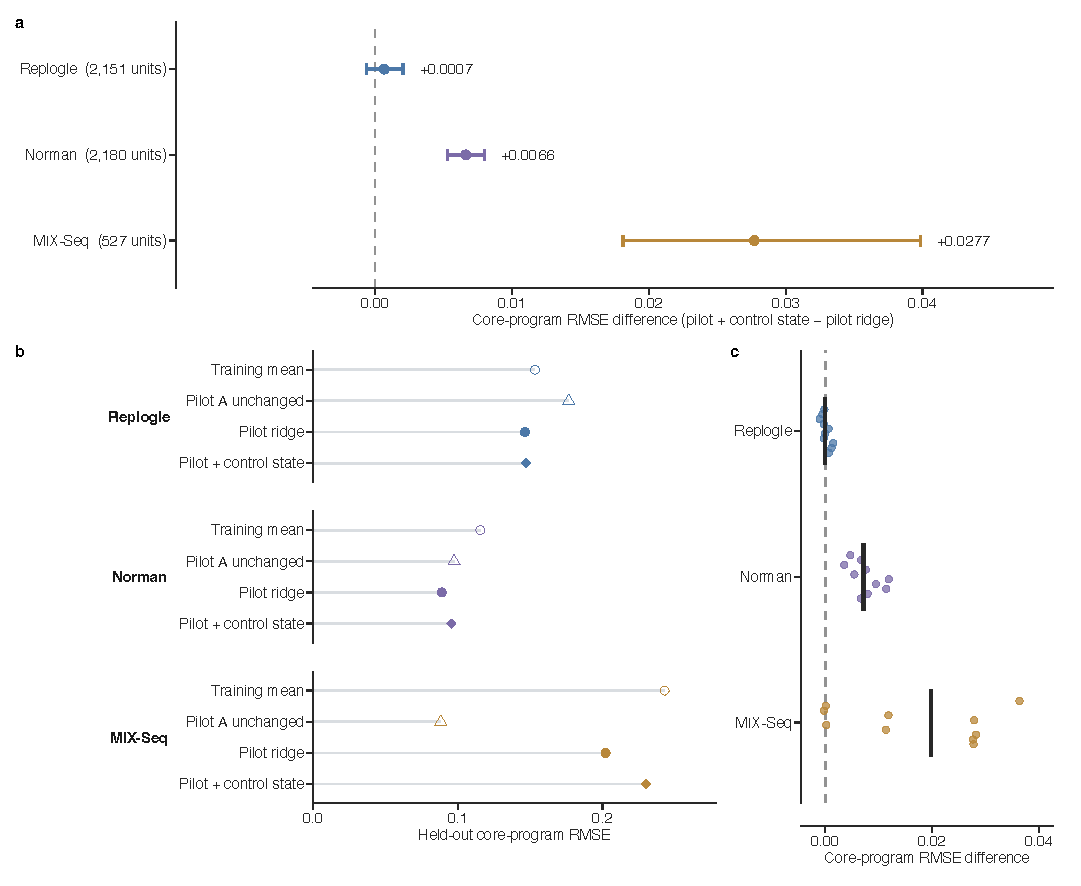
\includegraphics[width=\textwidth]{figure/Fig_cross_study_transfer.pdf}
\caption{\rev{\textbf{Matched control-state features do not improve the tested study-held-out response models.} \textbf{a}, Change in three-module response RMSE after adding independent control-state features to pilot-response ridge; positive values indicate worse prediction.} \rev{Intervals are conditional crossed intervention/context bootstrap intervals.} \rev{\textbf{b}, Absolute errors for simple and fitted comparators on identical eligible units.} \rev{\textbf{c}, Sensitivity across ten fixed random-cell partitions; the first partition is primary.} \rev{The held-out units comprise 527 MIX-Seq, 2,180 Norman and 2,151 Replogle perturbation--context observations.} \rev{Contexts and interventions recur across rows, GEMs are technical partitions, and bootstrap intervals do not quantify between-study replication.} \rev{The pilot is an observed response in a disjoint cell subset, not an exclusively pretreatment input.}}
\label{fig:transfer}
\end{figure}

\rev{The sampling-variance baseline also outperformed the learned disagreement models on primary log-disagreement RMSE in each held-out study (Supplementary Note S8).} \rev{Independent lineage data gave a compatible result under a different observation design.} \rev{In Schaff melanoma lineages, parent states were measured before a second treatment and descendants were linked by clone identity.} \rev{State-augmented ridge had standardized RMSE 0.9727, compared with 0.9663 for the training-selected treatment/count baseline; the full-refitting lineage-bootstrap difference was 0.00646 ($95\%$ interval $[-0.0111,0.0326]$).} \rev{A stricter support population likewise did not establish improvement (Supplementary Note S11).} \rev{These tests do not establish biological irrelevance of pretreatment state: genetic control-state variation is largely technical, and common intervention-specific descriptors were unavailable.} \rev{They did not demonstrate the proposed predictive gain in these measured settings.}

\FloatBarrier

\subsection{\rev{UPR effect ordering transfers where aggregate gene priority does not}}

\rev{We next asked whether a discovery-derived priority identified genes with reproducible program responses in separately generated studies.} \rev{The initial three-program score combined dominant effect, technical agreement and relative movement on the other programs.} \rev{Its fixed top-ten lists did not enrich the corresponding external responses.} \rev{In Adamson K562, top-ten mean sign-aligned standardized effect was 0.132, compared with 0.138 among the other twenty genes; the difference was $-0.0052$ ($95\%$ gene-bootstrap interval $[-0.165,0.145]$).} \rev{In unstimulated Frangieh melanoma, the difference was $-0.0386$ ($[-0.146,0.076]$).} \rev{The score did not outperform simple dominant-effect magnitude, and an integrated model-derived priority had insufficient common coverage and no demonstrated advantage (Supplementary Note S9).} \rev{Consequently, the coverage-derived gene hierarchy was not treated as a validated candidate-selection method.}

\rev{The subsequent axis-resolved comparison identified a narrower transferable feature.} \rev{Among all twelve axes and four external study-condition comparisons, UPR was the only axis with a significant positive association in both Adamson K562 and unstimulated Frangieh melanoma after joint correction across all 48 tests (Fig.~\ref{fig:upr-external}).} \rev{Source-versus-external UPR Spearman correlation was 0.823 in Adamson ($n=30$ genes; $95\%$ conditional interval $[0.639,0.916]$; $q=0.000960$) and 0.674 in unstimulated melanoma ($n=19$; interval $[0.275,0.904]$; $q=0.00840$).} \rev{The same melanoma genes did not support UPR correlation under interferon-$\gamma$ or co-culture.} \rev{However, direct paired comparisons between contexts did not survive multiplicity correction, so these data do not establish an immune-context interaction.}

\begin{figure}[tbp]
\centering
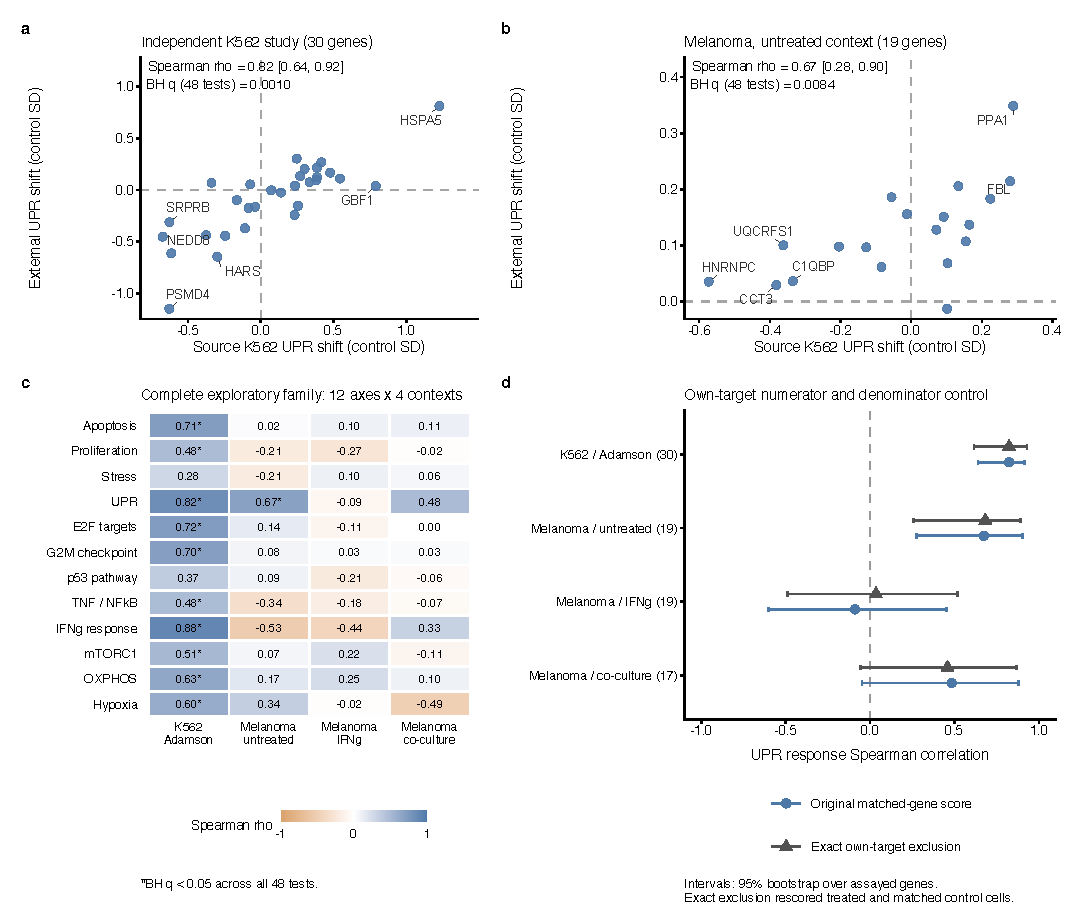
\includegraphics[width=\textwidth]{figure/Fig_UPR_external_validation.pdf}
\caption{\rev{\textbf{UPR effect ordering across independent perturbation studies.} \textbf{a,b}, Source Replogle K562 versus Adamson K562 (thirty genes) and unstimulated Frangieh melanoma (nineteen genes) UPR effects in the respective control-standard-deviation units.} \rev{All eligible genes are shown; labels identify six extreme effects in either context.} \rev{Dashed lines mark zero.} \rev{\textbf{c}, All twelve expression axes in Adamson and three melanoma contexts; asterisks indicate BH $q<0.05$ across all 48 comparisons.} \rev{\textbf{d}, Original and exact own-target numerator-and-denominator-corrected UPR correlations in each external context.} \rev{Bars are 95\% whole-gene bootstrap intervals from 2,000 draws.} \rev{Two-sided permutation tests use 10,000 draws; corrected UPR tests replace the four corresponding tests in a complete 48-test sensitivity family.} \rev{This axis-resolved follow-up is exploratory and tests relative ordering, rather than response-amplitude equivalence or a difference between contexts.}}
\label{fig:upr-external}
\end{figure}


\rev{The UPR ordering survived removal of the targeted gene from both the score numerator and its contribution to the common-library denominator: corrected correlations were 0.823 in Adamson and 0.682 in unstimulated melanoma.} \rev{Minimal covariate checks and leave-one-gene-out analyses retained positive point estimates, but equal-cell and single-guide resampling exposed lower precision in the small melanoma panel (Supplementary Note S9).} \rev{This was ordinal conservation rather than complete response-vector transfer.} \rev{Only nine of nineteen melanoma genes had source-concordant UPR effect signs, and copying the full twelve-axis source vector had higher RMSE than zero response in both external studies.} \rev{UPR therefore supplied a specific hypothesis for a new held-out-context test; it did not validate the aggregate priority or a universal response model.}

\FloatBarrier

\subsection{\rev{Source UPR priorities select relatively higher responses in a held-out cellular context}}

\rev{We tested the exploratory UPR result in Replogle RPE1 using a ranking fixed from K562 before RPE1 expression evaluation.} \rev{Metadata-defined support retained 438 shared target genes and 97,065 scored cells, including 11,485 non-targeting controls.} \rev{The common measurement space contained 6,780 genes and ninety UPR members.} \rev{Signed source--RPE1 effect correlation was $\rho=0.378$ ($95\%$ gene-bootstrap interval $[0.289,0.461]$; Holm-adjusted $P=0.000300$; Fig.~\ref{fig:upr-priority}).} \rev{It remained positive in the stricter 390-gene support population ($\rho=0.403$; interval $[0.307,0.496]$).} \rev{Thus the relative UPR-associated effects were reproducible across this cellular-context change, despite the absence of a successful shared baseline-state predictor.}

\rev{K562-defined quintiles supported an overall response gradient in RPE1 without a strictly monotonic increase in mean effect.} \rev{Mean effects from Q1 to Q5 were $-0.459$, $-0.170$, $-0.087$, $-0.038$ and $-0.068$ control standard deviations.} \rev{The Q5--Q1 contrast was 0.391 ($95\%$ gene-bootstrap interval $[0.266,0.521]$), the ordinal slope was 0.0915 per quintile ($[0.0639,0.1195]$), and Kendall's $\tau$ was 0.274; all three Holm-adjusted $P$ values were 0.000700.} \rev{Positive-effect fractions increased from 7/88 to 42/87, while the Q5--Q4 mean contrast was $-0.030$ (simultaneous $95\%$ interval $[-0.170,0.111]$).} \rev{Exact normalization and equal-cell sensitivities retained the broad gradient.} \rev{The evidence therefore supports enrichment of relatively higher and more often positive responses, rather than uniform activation or a stable increase between every adjacent quintile.}

\rev{The fixed top-twenty genes had a mean RPE1 UPR effect 0.329 control standard deviations above their one hundred matched background genes ($95\%$ matched-set bootstrap interval $[0.090,0.585]$; Holm-adjusted $P=0.000400$).} \rev{The nested top ten had a gap of 0.573 ($[0.217,0.965]$; adjusted $P=0.000400$).} \rev{These are relative response contrasts: the top-twenty mean itself was 0.044, compared with $-0.285$ in its background, and the top-ten mean was 0.243 versus $-0.330$.} \rev{The list therefore selects relatively higher UPR-associated expression, rather than uniformly activating UPR or producing stronger absolute perturbation effects.} \rev{Fourteen of twenty and nine of ten selected genes retained positive effects, but absolute-effect enrichment was uncertain (top-twenty $|d|$ gap 0.086; $95\%$ interval $[-0.041,0.214]$).} \rev{GBF1 and SPCS3 retained positive contrasts in RPE1 (0.934 and 0.795), whereas the ribosomal targets RPS13 and RPL7 reversed sign ($-1.145$ and $-1.335$).} \rev{Exact target-count exclusion from the normalization denominator retained the signed correlation ($\rho=0.378$) and matched gaps (0.328 and 0.572).} \rev{Equal-100-target-cell resampling also retained positive correlations and both matched gaps in every one of 200 draws (Supplementary Note S10).}

\begin{figure}[tbp]
\centering
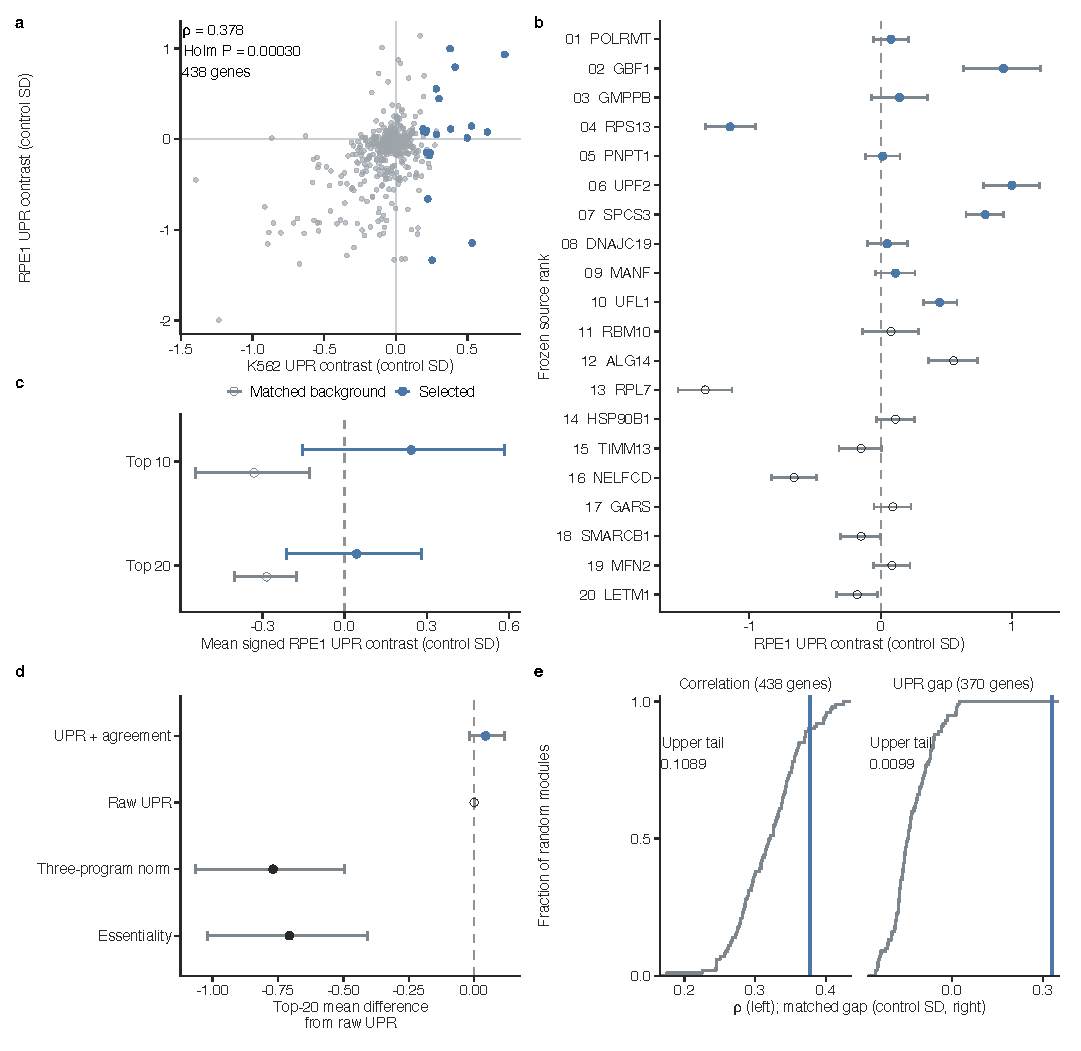
\includegraphics[width=\textwidth]{figure/Fig_UPR_RPE1_validation.pdf}
\caption{\rev{\textbf{Source-frozen UPR ordering and relative response prioritization in RPE1.} \textbf{a}, Signed K562 and RPE1 UPR effects across 438 fixed genes; blue marks the source top twenty.} \rev{\textbf{b}, All twenty priorities in fixed source order; filled points mark the first ten.} \rev{Bars are conditional 95\% shared-GEM wild intervals; GEMs are technical partitions.} \rev{\textbf{c}, Mean signed effects of selected genes and their frozen backgrounds, with 95\% intact-matched-set bootstrap intervals.} \rev{Selected-mean intervals span zero; matched signed gaps are positive.} \rev{\textbf{d}, Top-twenty mean differences from unweighted positive-UPR-effect ranking on the common 370-gene comparator population, with 95\% gene-bootstrap intervals.} \rev{The top-ten weighted and unweighted lists are identical. \textbf{e}, Empirical distributions for one hundred expression/detection-matched random modules; blue lines mark UPR.} \rev{Correlation specificity uses all 438 genes, while matched-utility specificity uses the uniform 370-gene complete-covariate sensitivity.} \rev{Only sixteen full-panel null lists have estimable utility matches.} \rev{All candidates and controls were fixed before RPE1 expression evaluation.} \rev{RPE1 is a held-out cellular context from the Replogle study, and the result concerns relative RNA-program effects.}}
\label{fig:upr-priority}
\end{figure}


\rev{The simple positive-UPR-effect ranking selected the same top-ten genes and gave similar top-twenty performance.} \rev{Agreement weighting did not demonstrate an additional benefit over that simple ranking: its top-twenty mean advantage was 0.044 ($95\%$ interval $[-0.018,0.117]$).} \rev{Generic transcriptional magnitude and essentiality selected different genes and yielded lower mean signed RPE1 UPR effects in the shared 370-gene comparator population.} \rev{Thus the measured discovery program, rather than a more complex model or generic perturbation strength, supplied the useful selection information.}

\rev{The fixed top-ten and top-twenty lists had Precision@10 of 0.90 and Precision@20 of 0.70, compared with 0.320 positive effects in the complete 438-gene panel and 0.28/0.23 in their matched backgrounds.} \rev{Continuous ranking quality did not improve over unweighted positive-source-UPR effects.} \rev{On the common comparator population, weighted versus unweighted NDCG@10 was 0.367 versus 0.436, and NDCG@20 was 0.337 versus 0.379.} \rev{Neither Precision nor NDCG differences supported a weighting advantage after the seven-test correction.} \rev{The two methods selected the same top ten but ordered them differently, illustrating why sign precision and magnitude-sensitive ranking are distinct outcomes.} \rev{Both UPR-based rankings had higher observed Precision and NDCG than the generic and random references for the specified Hallmark readout, with all reference distributions retained (Supplementary Note S12).} \rev{Conditioning on source and RPE1 mean log UMI counts retained descriptive matched gaps of 0.578 for the top ten ($95\%$ gene interval $[0.213,0.891]$) and 0.347 for the top twenty ($[0.073,0.592]$), without changing the candidate lists or sign criterion.}

\rev{The random-module controls delimit this result.} \rev{UPR's source--RPE1 rank correlation was not exceptional among one hundred expression/detection-matched random modules (upper-tail fraction 0.109).} \rev{On the complete-covariate population, however, the actual UPR priorities gave a larger matched gap on the RPE1 UPR outcome than every random-module priority (finite-null upper-tail fraction $1/101=0.00990$; two-comparison Holm-adjusted value 0.0198).} \rev{The full 438-gene primary panel had only sixteen estimable matched-null lists, so it could not establish the same specificity ($1/17=0.0588$).} \rev{This supports program-directed selection within the complete-covariate population, while providing no evidence that UPR is uniquely conserved genome-wide.} \rev{Removing each of the ninety readout genes in turn retained a positive top-twenty matched gap (range 0.305--0.341).} \rev{All fixed lists, background genes, individual effects and failed-null availability are retained in Supplementary Note S10 and Supplementary Data.}

\FloatBarrier

\rev{Curated readouts and matched random modules did not establish UPR-specific conservation.} \rev{None of eight predefined RNA readouts had an RPE1 ordering association exceptional relative to its size/expression/detection-matched random sets (upper-tail fractions 0.267--1.000), and the Hallmark-disjoint Reactome readout failed to retain the source--RPE1 association ($\rho=-0.024$; BH $q=0.760$).} \rev{Alternative definitions also changed candidate rankings.} \rev{These negative controls restrict the interpretation to response ordering and selection for a specified transcriptional readout; full module results and the curated-readout figure are retained in Supplementary Note S13 and Fig.~S15.}

\subsection{\rev{An independent screen preserves ordering, with lower-support evidence for fixed-list utility}}

\rev{The frozen UPR readout retained positive ordering in the newly evaluated HepG2 screen (Fig.~\ref{fig:hepg2-independent}).} \rev{Among the 417 perturbations meeting primary support, source--HepG2 Spearman correlation was 0.403 ($95\%$ whole-gene interval $[0.313,0.489]$; Holm-adjusted $P=0.00050$).} \rev{Direction concordance was 63.5\%.} \rev{The fixed-library sensitivity gave $\rho=0.404$, and the hundred-cell subset retained $\rho=0.449$ ($[0.265,0.601]$).} \rev{Thus the response-order association extended to a separately generated experiment without fitting to its outcomes.}

\rev{The full candidate lists required a different evidential qualification.} \rev{GBF1 and ALG14 had seventeen and twenty-four cells, respectively; the primary top-ten/top-twenty utility tests were therefore unestimable.} \rev{In the separately specified ten-cell sensitivity, the unchanged lists contained eight and fifteen positive effects.} \rev{Mean effects were 0.394 and 0.220 control standard deviations, compared with $-0.117$ and $-0.121$ among the remaining genes.} \rev{Corresponding signed gaps were 0.511 ($95\%$ gene interval $[0.282,0.734]$) and 0.341 ($[0.191,0.493]$).} \rev{Shared-GEM sensitivity ranges also remained positive.} \rev{These results provide independent-screen selection evidence at lower cell support, rather than successful primary validation of both complete lists.}

\rev{On the common 370-gene comparison frame, Precision@10/@20 was 0.80/0.75, against a positive-effect prevalence of 123/370.} \rev{Weighted NDCG was 0.574/0.525, whereas simple source-UPR ordering gave 0.594/0.565 with the same sign precision.} \rev{Both program-directed rankings exceeded the observed generic-strength, essentiality and expression baselines.} \rev{The weighted lists also exceeded all one hundred matched-module priorities on Precision and NDCG (descriptive upper-tail fractions $1/101$).} \rev{The independent data therefore support relative selection for the specified transcriptional readout, with no observed ranking benefit from agreement weighting; stringent complete-list support and functional intervention benefit remain separate requirements.}

\begin{figure}[tbp]
\centering
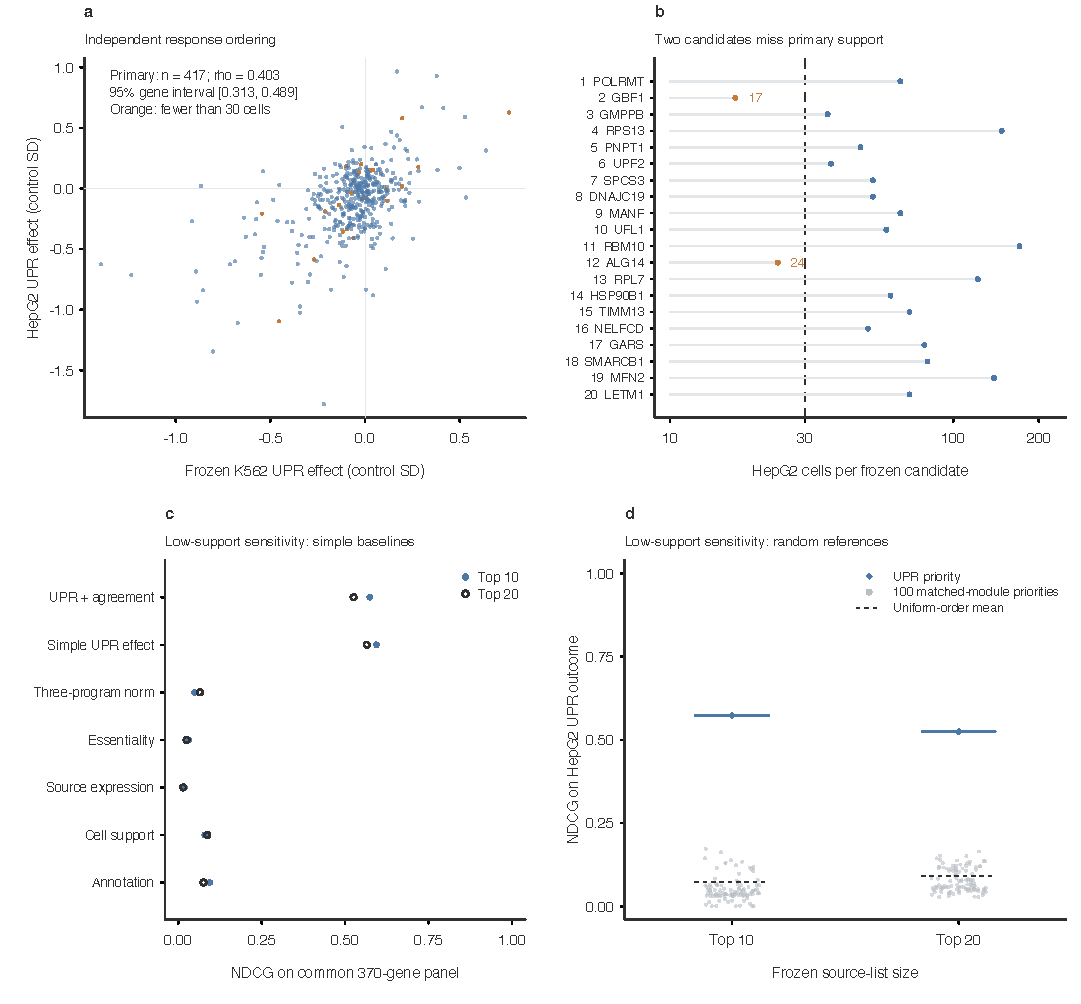
\includegraphics[width=\textwidth]{figure/Fig_UPR_independent_HepG2.pdf}
\caption{\rev{\textbf{Independent HepG2 evaluation separates ordering from complete-list support.} \textbf{a}, Frozen source effects versus exact-composition-corrected HepG2 UPR effects for all 438 genes; orange points have fewer than thirty target cells.} \rev{The correlation and 95\% whole-gene interval refer to the 417-gene primary panel.} \rev{\textbf{b}, Cell support for all twenty frozen candidates in source-priority order; the dashed line marks the primary threshold.} \rev{GBF1 and ALG14 prevent primary evaluation of the complete lists.} \rev{\textbf{c,d}, Separately specified ten-cell sensitivity on the unchanged 370-gene complete-source-covariate frame.} \rev{Filled/open points in c denote top-ten/top-twenty NDCG.} \rev{Panel d shows all one hundred matched-module source priorities evaluated on the same HepG2 UPR outcome; blue diamonds and horizontal marks denote observed UPR-priority values, not uncertainty bars, and dotted segments denote uniform-order means.} \rev{All source rankings, readout members, $K$, sign threshold and gain definition were fixed before expression scoring.} \rev{Lower-support results are secondary evidence and do not replace the missing primary list tests.} \rev{Effects summarize RNA expression, not pathway flux or functional benefit.}}
\label{fig:hepg2-independent}
\end{figure}

\FloatBarrier

\section{Discussion}

\rev{The principal finding is that reproducible ordering of transcriptional program responses can inform candidate perturbation prioritization across experimental contexts.} \rev{UPR-associated gene-effect ordering persisted across separately generated K562 and unstimulated melanoma screens, survived direct target-expression composition controls, and extended to source-frozen RPE1 and independent HepG2 evaluations.} \rev{Ordering and selection provide complementary evidence: RPE1 priorities selected relatively higher responses on the specified RNA program, whereas HepG2 confirmed ordering under the primary support rule and supplied secondary, lower-support evidence for the unchanged candidate lists.} \rev{This establishes an experimentally testable use of cross-resource transcriptional measurements: prioritizing perturbations for a defined program response in another cellular context.} \rev{Its scope is response ranking and molecular-screen selection, with complete-list primary validation governed by cell coverage.}

\rev{The biological interpretation builds on the original screens.} \rev{Adamson established genetic dissection of the UPR, and Replogle distinguished canonical ER-associated UPR from integrated stress responses associated with mitochondrial and translational perturbations.~\cite{adamson2016,replogle2022}} \rev{The distinction between a coherent expression signature and an annotated functional process matters here: Hallmark signatures, Reactome pathway participants and GO process members summarize different gene collections.~\cite{liberzon2015,go2000,go2026,reactome2024}} \rev{Positive correlations for several curated readouts survived removal of Hallmark overlap, but their RPE1 correlations were not exceptional relative to matched random sets.} \rev{The failed Hallmark-disjoint Reactome readout and the non-invariant candidate lists therefore limit interpretation to a defined RNA response, rather than a uniquely conserved UPR mechanism.} \rev{The fixed RPE1 priorities include GBF1, SPCS3 and HSP90B1 alongside POLRMT and PNPT1, consistent with perturbations affecting several aspects of protein handling and organelle function.} \rev{Replogle's analysis already connected mitochondrial RNA regulation to cellular stress.~\cite{replogle2022}} \rev{The present evidence adds a cross-context test of relative program effects and a bounded gene-selection result; it does not identify a new UPR mechanism.} \rev{The lack of a corrected melanoma context difference also prevents attributing the observed association pattern to immune-induced rewiring.~\cite{frangieh2021}}

\rev{The distinction between ordering and calibration matters for prediction.} \rev{Full response-vector copying performed poorly in external studies, and matched control-state features did not improve the tested study-held-out models.} \rev{These findings are compatible with methods that perform well in other, explicitly defined prediction settings, including scGen, CPA, chemCPA and GEARS, and with the need for task-matched benchmarks.~\cite{scgen2019,cpa2023,chemcpa2022,gears2024,benchmark2026}} \rev{Systema showed that systematic variation can inflate apparent genetic-response prediction performance.~\cite{systema2026}} \rev{Here, expression-matched random modules also showed substantial cross-context correlation, so correlation alone cannot establish UPR-specific biological conservation.} \rev{The more informative distinction was selection for the specified UPR outcome: generic response magnitude, essentiality and matched random-program priorities did not select the same relative responses.} \rev{Positive-effect precision and magnitude-sensitive ranking answer different selection questions.} \rev{The fixed lists enriched positive RNA responses, but agreement weighting did not improve NDCG over unweighted source effects and alternative definitions changed the selected genes.} \rev{Their practical value is consequently conditional on the specified RNA readout; neither a general algorithmic advantage nor functional intervention benefit follows.}

\rev{Nadig and colleagues previously documented broad differential-expression sharing across cellular contexts.~\cite{nadig2025}} \rev{The HepG2 result extends our ordering and source-frozen selection evaluation to a separately generated screen; it does not make generic response conservation a new UPR mechanism.} \rev{Positive lower-support effects for candidates spanning protein handling and mitochondrial RNA regulation are consistent with the heterogeneous stress responses described in the original screens.~\cite{adamson2016,replogle2022}} \rev{The useful information was the measured response on the chosen RNA program: both weighted and simple program-effect rankings selected higher corresponding responses than generic-strength and random-module priorities.} \rev{Seventeen GBF1 cells and twenty-four ALG14 cells nevertheless leave complete-list primary validation unresolved.} \rev{The distinction is consequential: observed lower-support enrichment can guide a molecular screen, but cannot substitute for adequate independent support or a functional phenotype.}

Culture context and baseline heterogeneity are associated with changes in clonal output and stress-related transcription, making several biological explanations plausible.~\cite{weinreb2020,lyu2026serum,lyu2026stress} \rev{Our context features were matched-horizon controls, whereas the independent lineage experiment measured earlier relatives before a second intervention.} \rev{Neither analysis established a general predictive gain from the tested state features.} \rev{This does not contradict the original lineage studies' evidence that clonal states and treatment history influence later outcomes.~\cite{weinreb2020,schaff2024}} \rev{The experiments ask different questions and resolve different units.} \rev{In particular, technical control-state variation in pooled genetic screens cannot estimate how an individual cell's pretreatment state causally modifies its perturbation response.} \rev{The new results support transport of measured program information across the tested contexts, without establishing that transport is caused by a shared baseline-state mechanism.}

\rev{The validation scope remains specific.} \rev{Adamson was enriched for UPR-related perturbations, the independent melanoma panel was small and sampling sensitive, and RPE1 was a different cellular context within the Replogle study.} \rev{The UPR holdout was specified after the complete exploratory axis analysis, and the complete-covariate random-module test is a sensitivity population, not a replacement for the primary panel.} \rev{The additional module and ranking checks used already examined outcomes, with definitions and metrics fixed before their corresponding calculations; they provide robustness evidence rather than a new untouched validation.} \rev{The subsequent HepG2 screen was reserved before expression scoring and supplies an unused cross-study test; its lower-support list sensitivity remains distinct from the unestimable primary list endpoints.} \rev{Conditional gene and technical resampling do not supply independent culture replication.} \rev{RNA-program effects also do not measure death, division or stable fate commitment; complementary molecular and functional assays are needed to establish a signalling mechanism or beneficial intervention.~\cite{adamson2016,replogle2022,cahan2014,rackham2016}} \rev{Within these bounds, the fixed gene lists and comparator results provide a reproducible starting point for selecting relatively preserved or elevated UPR-associated expression responses across cellular backgrounds.}

\section{Conclusions}

\rev{The Hallmark-defined UPR-associated RNA contrast retains a relative ordering across the tested genetic contexts, with extension to other curated readouts depending on definition and background.} \rev{A source-frozen program ranking enriches the corresponding signed response in RPE1, with no demonstrated ranking benefit from agreement weighting over positive source effects alone.} \rev{Independent HepG2 data reinforce response-order transport and provide secondary selection evidence, while complete-list primary utility remains coverage-limited.} \rev{The supported contribution is relative prioritization for defined RNA readouts; UPR-specific regulation, calibrated whole-response prediction and a general baseline-state mechanism remain unestablished.}

\section*{Supplementary material}

\rev{Supplementary materials provide common feature definitions, full validation results, sampling and normalization sensitivities, fixed candidate lists and supporting assay-specific analyses.} \rev{Machine-readable effects, predictions, matched backgrounds and random-module comparisons accompany the Supplementary Data; the complete executable analysis and processed inputs are supplied separately.}

\section*{Ethics statement}
Not applicable. This study was a secondary analysis of publicly available, de-identified datasets and involved no new recruitment of human participants, use of identifiable human data or tissue, animal experimentation, intervention or biological sample collection. Ethics approval and informed consent for the original studies were reported by the respective data-generating investigators.

\section*{Data availability}
\rev{No new biological data were generated.} \rev{Public sources are Replogle K562 and RPE1 Perturb-seq, Figshare article 20029387 (\url{https://doi.org/10.6084/m9.figshare.20029387}); Norman CRISPRa, GSE133344 (\url{https://www.ncbi.nlm.nih.gov/geo/query/acc.cgi?acc=GSE133344}); MIX-Seq, Figshare version 3 (\url{https://doi.org/10.6084/m9.figshare.10298696.v3}); Adamson CRISPRi, GSE90546/GSM2406681 (\url{https://www.ncbi.nlm.nih.gov/geo/query/acc.cgi?acc=GSE90546}); Frangieh CRISPR knockout, SCP1064 (\url{https://singlecell.broadinstitute.org/single_cell/study/SCP1064}); and Schaff lineage tracing, GSE253739 (\url{https://www.ncbi.nlm.nih.gov/geo/query/acc.cgi?acc=GSE253739}).} \rev{Independent HepG2 validation uses GSE264667 (\url{https://www.ncbi.nlm.nih.gov/geo/query/acc.cgi?acc=GSE264667}).} \rev{Supporting analyses additionally use LARRY, GSE140802, and MultiPerturb, GSE277747.} \rev{The generic essentiality comparator is from DepMap Public 24Q4 (\url{https://doi.org/10.25452/figshare.plus.27993248.v1}).} \rev{Original matrices are identified by accession, feature schema and checksum rather than duplicated.}

\rev{The source-analysis code, processed inputs, validation splits and software records are publicly available at \url{https://github.com/azusakou/State-dependent-response-geometry}.} \rev{The accompanying reproducibility archive supplies the harmonized count-scoring workflow, frozen feature and eligibility definitions, disjoint cell partitions, study-held-out predictions, independent-study validation, source-frozen RPE1 analysis, complete random-module controls and figure source tables.} \rev{It additionally provides the authoritative functional memberships, alternate-definition scores, quintile and ranking checks, execution logs and figure source tables.} \rev{It also retains the supporting sampling-simulation and intervention-choice analyses.} \rev{These additional files are supplied with the article separately from the existing repository.} \rev{Compact endpoint, candidate, matching, sensitivity and null-result tables are provided as Supplementary Data.}

\section*{Declaration of competing interest}
The authors declare that they have no competing interests.

\section*{Funding}
The authors received no specific funding for this work.

\printcredits

\section*{Acknowledgements}
The authors thank the investigators who generated and publicly shared the datasets used in this study.

\begingroup
\color{black}
\colorlet{scolor}{black}
\hypersetup{citecolor=black,linkcolor=black,urlcolor=black}
\begin{thebibliography}{99}
\bibitem{takahashi2006}
K.~Takahashi, S.~Yamanaka, Induction of pluripotent stem cells from mouse embryonic and adult fibroblast cultures by defined factors, Cell 126 (2006) 663--676.
\newblock \href {https://doi.org/10.1016/j.cell.2006.07.024} {\path{doi:10.1016/j.cell.2006.07.024}}.

\bibitem{cahan2014}
P.~Cahan, H.~Li, S.~A. Morris, E.~Lummertz~da Rocha, G.~Q. Daley, J.~J. Collins, {CellNet}: network biology applied to stem cell engineering, Cell 158 (2014) 903--915.
\newblock \href {https://doi.org/10.1016/j.cell.2014.07.020} {\path{doi:10.1016/j.cell.2014.07.020}}.

\bibitem{rackham2016}
O.~J.~L. Rackham, J.~Firas, H.~Fang, M.~E. Oates, M.~L. Holmes, A.~S. Knaupp, et~al., A predictive computational framework for direct reprogramming between human cell types, Nature Genetics 48 (2016) 331--335.
\newblock \href {https://doi.org/10.1038/ng.3487} {\path{doi:10.1038/ng.3487}}.

\bibitem{kamimoto2023}
K.~Kamimoto, B.~Stringa, C.~M. Hoffmann, K.~Jindal, L.~Solnica-Krezel, S.~A. Morris, Dissecting cell identity via network inference and in silico gene perturbation, Nature 614 (2023) 742--751.
\newblock \href {https://doi.org/10.1038/s41586-022-05688-9} {\path{doi:10.1038/s41586-022-05688-9}}.

\bibitem{dix2016}
A.~Dixit, O.~Parnas, B.~Li, J.~Chen, C.~P. Fulco, L.~Jerby-Arnon, et~al., {Perturb-Seq}: dissecting molecular circuits with scalable single-cell {RNA} profiling of pooled genetic screens, Cell 167 (2016) 1853--1866.e17.
\newblock \href {https://doi.org/10.1016/j.cell.2016.11.038} {\path{doi:10.1016/j.cell.2016.11.038}}.

\bibitem{adamson2016}
B.~Adamson, T.~M. Norman, M.~Jost, M.~Y. Cho, J.~K. Nu{\~n}ez, Y.~Chen, et~al., A multiplexed single-cell {CRISPR} screening platform enables systematic dissection of the unfolded protein response, Cell 167 (2016) 1867--1882.e21.
\newblock \href {https://doi.org/10.1016/j.cell.2016.11.048} {\path{doi:10.1016/j.cell.2016.11.048}}.

\bibitem{jaitin2016}
D.~A. Jaitin, A.~Weiner, I.~Yofe, D.~Lara-Astiaso, H.~Keren-Shaul, E.~David, et~al., Dissecting immune circuits by linking {CRISPR}-pooled screens with single-cell {RNA-seq}, Cell 167 (2016) 1883--1896.e15.
\newblock \href {https://doi.org/10.1016/j.cell.2016.11.039} {\path{doi:10.1016/j.cell.2016.11.039}}.

\bibitem{datlinger2017}
P.~Datlinger, A.~F. Rendeiro, C.~Schmidl, T.~Krausgruber, P.~Traxler, J.~Klughammer, et~al., Pooled {CRISPR} screening with single-cell transcriptome readout, Nature Methods 14 (2017) 297--301.
\newblock \href {https://doi.org/10.1038/nmeth.4177} {\path{doi:10.1038/nmeth.4177}}.

\bibitem{gasperini2019}
M.~Gasperini, A.~J. Hill, J.~L. McFaline-Figueroa, B.~Martin, S.~Kim, M.~D. Zhang, et~al., A genome-wide framework for mapping gene regulation via cellular genetic screens, Cell 176 (2019) 377--390.e19.
\newblock \href {https://doi.org/10.1016/j.cell.2018.11.029} {\path{doi:10.1016/j.cell.2018.11.029}}.

\bibitem{schraivogel2020}
D.~Schraivogel, A.~R. Gschwind, J.~H. Milbank, D.~R. Leonce, P.~Jakob, L.~Mathur, et~al., Targeted {Perturb-seq} enables genome-scale genetic screens in single cells, Nature Methods 17 (2020) 629--635.
\newblock \href {https://doi.org/10.1038/s41592-020-0837-5} {\path{doi:10.1038/s41592-020-0837-5}}.

\bibitem{replogle2022}
J.~M. Replogle, R.~A. Saunders, A.~N. Pogson, J.~A. Hussmann, A.~Lenail, A.~Guna, et~al., Mapping information-rich genotype--phenotype landscapes with genome-scale {Perturb-seq}, Cell 185 (2022) 2559--2575.e28.
\newblock \href {https://doi.org/10.1016/j.cell.2022.05.013} {\path{doi:10.1016/j.cell.2022.05.013}}.

\bibitem{norman2019}
T.~M. Norman, M.~A. Horlbeck, J.~M. Replogle, A.~Y. Ge, A.~Xu, M.~Jost, et~al., Exploring genetic interaction manifolds constructed from rich single-cell phenotypes, Science 365 (2019) 786--793.
\newblock \href {https://doi.org/10.1126/science.aax4438} {\path{doi:10.1126/science.aax4438}}.

\bibitem{mcfarland2020}
J.~M. McFarland, B.~R. Paolella, A.~Warren, K.~Geiger-Schuller, T.~Shibue, M.~Rothberg, et~al., Multiplexed single-cell transcriptional response profiling to define cancer vulnerabilities and therapeutic mechanism of action, Nature Communications 11 (2020) 4296.
\newblock \href {https://doi.org/10.1038/s41467-020-17440-w} {\path{doi:10.1038/s41467-020-17440-w}}.

\bibitem{scgen2019}
M.~Lotfollahi, F.~A. Wolf, F.~J. Theis, {scGen} predicts single-cell perturbation responses, Nature Methods 16 (2019) 715--721.
\newblock \href {https://doi.org/10.1038/s41592-019-0494-8} {\path{doi:10.1038/s41592-019-0494-8}}.

\bibitem{cpa2023}
M.~Lotfollahi, A.~Klimovskaia~Susmelj, C.~De~Donno, L.~Hetzel, Y.~Ji, I.~L. Ibarra, et~al., Predicting cellular responses to complex perturbations in high-throughput screens, Molecular Systems Biology 19 (2023) e11517.
\newblock \href {https://doi.org/10.15252/msb.202211517} {\path{doi:10.15252/msb.202211517}}.

\bibitem{chemcpa2022}
L.~Hetzel, S.~B{\"o}hm, N.~Kilbertus, S.~G{\"u}nnemann, M.~Lotfollahi, F.~J. Theis, Predicting cellular responses to novel drug perturbations at a single-cell resolution, in: Advances in Neural Information Processing Systems, Vol.~35, 2022, pp. 26711--26722.

\bibitem{gears2024}
Y.~Roohani, K.~Huang, J.~Leskovec, Predicting transcriptional outcomes of novel multigene perturbations with {GEARS}, Nature Biotechnology 42 (2024) 927--935.
\newblock \href {https://doi.org/10.1038/s41587-023-01905-6} {\path{doi:10.1038/s41587-023-01905-6}}.

\bibitem{systema2026}
\rev{R.~Vi\~nas Torn\'e, M.~Wiatrak, Z.~Piran, S.~Fan, L.~Jiang, S.~A.~Teichmann, M.~Nitzan, M.~Brbi\'c, Systema: a framework for evaluating genetic perturbation response prediction beyond systematic variation, Nature Biotechnology 44 (2026) 1050--1059.
\newblock \href{https://doi.org/10.1038/s41587-025-02777-8}{\path{doi:10.1038/s41587-025-02777-8}}.}

\bibitem{weinreb2020}
C.~Weinreb, A.~Rodriguez-Fraticelli, F.~D. Camargo, A.~M. Klein, Lineage tracing on transcriptional landscapes links state to fate during differentiation, Science 367 (2020) eaaw3381.
\newblock \href {https://doi.org/10.1126/science.aaw3381} {\path{doi:10.1126/science.aaw3381}}.

\bibitem{biddy2018}
B.~A. Biddy, W.~Kong, K.~Kamimoto, C.~Guo, S.~E. Waye, T.~Sun, et~al., Single-cell mapping of lineage and identity in direct reprogramming, Nature 564 (2018) 219--224.
\newblock \href {https://doi.org/10.1038/s41586-018-0744-4} {\path{doi:10.1038/s41586-018-0744-4}}.

\bibitem{kester2018}
L.~Kester, A.~van Oudenaarden, Single-cell transcriptomics meets lineage tracing, Cell Stem Cell 23 (2018) 166--179.
\newblock \href {https://doi.org/10.1016/j.stem.2018.04.014} {\path{doi:10.1016/j.stem.2018.04.014}}.

\bibitem{schaff2024}
\rev{D.~L.~Schaff, A.~J.~Fasse, P.~E.~White, R.~J.~Vander Velde, S.~M.~Shaffer, Clonal differences underlie variable responses to sequential and prolonged treatment, Cell Systems 15 (2024) 213--226.e9.
\newblock \href{https://doi.org/10.1016/j.cels.2024.01.011}{\path{doi:10.1016/j.cels.2024.01.011}}.}

\bibitem{frangieh2021}
C.~J. Frangieh, J.~C. Melms, P.~I. Thakore, K.~R. Geiger-Schuller, P.~Ho, A.~M. Luoma, et~al., Multimodal pooled {Perturb-CITE-seq} screens in patient models define mechanisms of cancer immune evasion, Nature Genetics 53 (2021) 332--341.
\newblock \href {https://doi.org/10.1038/s41588-021-00779-1} {\path{doi:10.1038/s41588-021-00779-1}}.

\bibitem{liberzon2015}
A.~Liberzon, C.~Birger, H.~Thorvaldsd{\'o}ttir, M.~Ghandi, J.~P. Mesirov, P.~Tamayo, The molecular signatures database hallmark gene set collection, Cell Systems 1 (2015) 417--425.
\newblock \href {https://doi.org/10.1016/j.cels.2015.12.004} {\path{doi:10.1016/j.cels.2015.12.004}}.

\bibitem{depmap2024}
\rev{Broad DepMap, DepMap 24Q4 Public, Figshare+ (2024).
\newblock \href{https://doi.org/10.25452/figshare.plus.27993248.v1}{\path{doi:10.25452/figshare.plus.27993248.v1}}.}

\bibitem{dempster2021}
\rev{J.~M.~Dempster, I.~Boyle, F.~Vazquez, D.~E.~Root, J.~S.~Boehm, W.~C.~Hahn, A.~Tsherniak, J.~M.~McFarland, Chronos: a cell population dynamics model of CRISPR experiments that improves inference of gene fitness effects, Genome Biology 22 (2021) 343.
\newblock \href{https://doi.org/10.1186/s13059-021-02540-7}{\path{doi:10.1186/s13059-021-02540-7}}.}

\bibitem{go2000}
\rev{M.~Ashburner, C.~A.~Ball, J.~A.~Blake, D.~Botstein, H.~Butler, J.~M.~Cherry, et~al., Gene ontology: tool for the unification of biology, Nature Genetics 25 (2000) 25--29.
\newblock \href{https://doi.org/10.1038/75556}{\path{doi:10.1038/75556}}.}

\bibitem{go2026}
\rev{The Gene Ontology Consortium, The Gene Ontology knowledgebase in 2026, Nucleic Acids Research 54 (2026) D1779--D1792.
\newblock \href{https://doi.org/10.1093/nar/gkaf1292}{\path{doi:10.1093/nar/gkaf1292}}.}

\bibitem{reactome2024}
\rev{M.~Milacic, D.~Beavers, P.~Conley, C.~Gong, M.~Gillespie, J.~Griss, et~al., The Reactome Pathway Knowledgebase 2024, Nucleic Acids Research 52 (2024) D672--D678.
\newblock \href{https://doi.org/10.1093/nar/gkad1025}{\path{doi:10.1093/nar/gkad1025}}.}

\bibitem{nadig2025}
\rev{A.~Nadig, J.~M.~Replogle, A.~N.~Pogson, V.~Murthy, S.~A.~McCarroll, J.~S.~Weissman, et~al., Transcriptome-wide analysis of differential expression in perturbation atlases, Nature Genetics 57 (2025) 1228--1237.
\newblock \href{https://doi.org/10.1038/s41588-025-02169-3}{\path{doi:10.1038/s41588-025-02169-3}}.}

\bibitem{benchmark2026}
Z.~Wei, Y.~Wang, Y.~Gao, S.~Wang, P.~Li, D.~Si, et~al., Benchmarking algorithms for generalizable single-cell perturbation response prediction, Nature Methods 23 (2026) 451--464.
\newblock \href {https://doi.org/10.1038/s41592-025-02980-0} {\path{doi:10.1038/s41592-025-02980-0}}.

\bibitem{lyu2026serum}
Z.~Lyu, C.~Shao, R.~Yang, Q.~Yu, M.~Yang, G.~Yang, Z.~Wang, Serum withdrawal establishes a stress-dominant entry state during myogenic differentiation, Frontiers in Cell and Developmental Biology 14 (2026) 1823860.
\newblock \href {https://doi.org/10.3389/fcell.2026.1823860} {\path{doi:10.3389/fcell.2026.1823860}}.

\bibitem{lyu2026stress}
Z.~Lyu, C.~Shao, R.~Yang, Q.~Yu, G.~Yang, Z.~Wang, Pre-Existing Heterogeneity Predicts Rare Proteostasis-Stress Programs Across Diverse Perturbations, Biology 15 (2026) 1230.
\newblock \href {https://doi.org/10.3390/biology15151230} {\path{doi:10.3390/biology15151230}}.
\end{thebibliography}
\endgroup
\end{document}
